\chapter{Решение} \label{chapt3}

\section{Получение данных} \label{sect3_1}
Для решения задачи классификации нейронной сетью требуется наличие данных для обучения. Датасетов с настоящей проблемой в открытом доступе не нашлось, поэтому данные пришлось получать вручную.

\begin{figure}[ht] 
  \center
  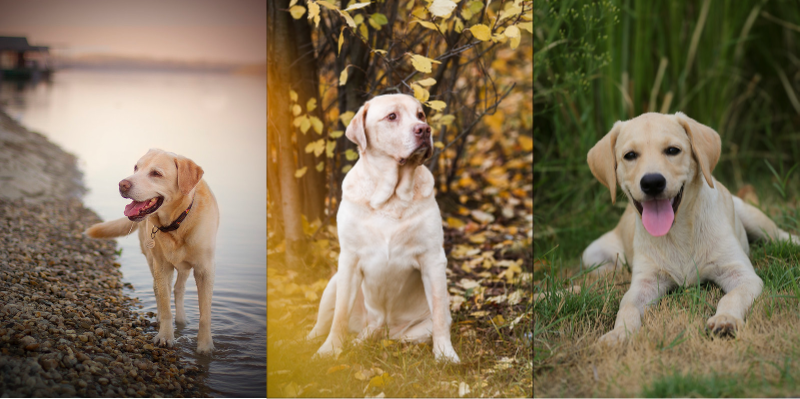
\includegraphics [width=\textwidth*2/3] {dogs-classes}
  \caption{Позы собаки, на которые классифицируются изображения: собака стоит, собака сидит и собака лежит} 
  \label{img:classes}  
\end{figure}

\subsection{Первая итерация} \label{subsect3_1_1}
За основу был взят датасет OpenImageDataset[2] - набор изображений на более чем тысячу разных классов. Из него был взят подкласс Dog, в котором было 20000 изображений собак. Далее эти данные были размечены на Яндекс.Толоке. Каждое изображение было показано пользователю Толоки с вопросом “В какой позиции собака находится на этом фото”. Фотографии были размечены с пятикратным перекрытием, т.е. каждое изображение размечалось пять раз разными людьми.
На выходе получился скромного размера датасет, часть изображений в нём не подходили под постановку задач, но на выходе имелась следующая информация:
\begin{enumerate}
    \item Поза собаки (стоит, сидит, лежит на спине, лежит на боку)
    \item Поза хвоста собаки (вверх, вниз, прямо)
    \item Рот собаки (открыт, закрыт, высунут язык)
    \item Уши собаки (торчат, опущены)
    \item Количество собак в кадре
    \item Загорожена ли собака в кадре
    \item Ограничивающая рамка (bounding box) вокруг собаки.
    \item Ограничивающая рамка ушей, хвоста и рта собаки.
\end{enumerate}

\subsection{Создание эталонного датасета} \label{subsect3_1_2}
Учитывая прошлые ошибки было принято решение собрать датасет заново, используя опыт, полученный при разметке первого.

Главные изменения заключаются в следующем:
\begin{enumerate}
    \item Датасет собирается итеративно по небольшим частям и выводы делаются сразу
    \item Размер каждого класса удерживается на одинаковом уровне
    \item Проводится учёт всех изображений, которые тяжело размечать
\end{enumerate}{}

В статье Amy Bearman и Cathering Dong \cite{Bearman2015HumanPE} указывается что нейронным сетям тяжело распознать позу, при наличии окклюзий, поворотов и переворотов, сильных перспективных искажений, и множественных объектов. В новом датасете было уделено особое внимание трудноклассифицируемым изображениям, поэтому они всячески избегались.

\begin{figure}[ht] 
  \center
  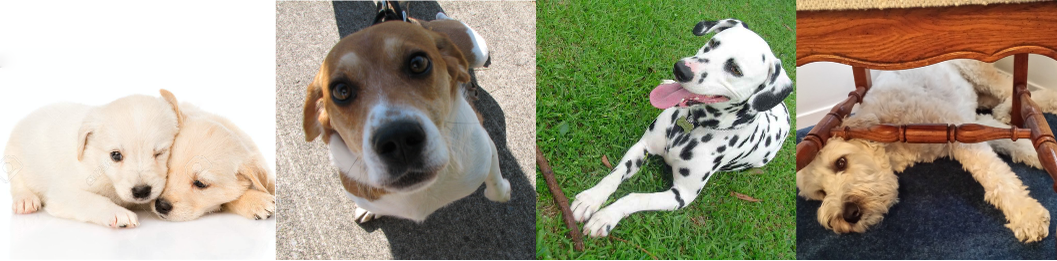
\includegraphics [width=\textwidth] {hazards_dogs}
  \caption{Позы, которые трудно определить: множественные объекты, перспективные искажения, повороты и окклюзии} 
  \label{img:hazards_dogs}  
\end{figure}

На этот раз источником изображений был Flickr. В нём содержится множество фотографий, который можно было фильтровать как по ориентации - только вертикальные, например. По породе - можно явно указать, что мы ищем Лабрадора Ретривера. Либо только снятые на телефон. В общем, сильно больше контроля при выборе фотографий.

В итоге были собраны изображения собак по 100 изображений на целевой класс. На них была обучена простейшая архитектура, т.н. ShallowNet с одним свёрточным слоем.
Результаты следующие:
\begin{itemize}
    \item При классификации «в лоб» достигается точность в 60\%
    \item При обрезании изображений по ограничительной рамке собаки, точность увеличивается до 68\%
    \item При использовании черно-белых изображений точность также возрастает до 68\%
\end{itemize}

\subsection{Фильтрация исходного датасета} \label{subsect3_1_2}
Собирать фотографии заново было достаточно хорошим упражнением, но главной проблемой были огромные временные затраты на создание датасета даже с 300 фотографиями. Более того, из 80000 фотографий по тегу Лабрадор Ретривер, автором и его ассистентом было просмотрено 70000 из них. И уже из них были собраны те 300 фотографий.
В итоге было принято решение просмотреть исходный датасет и повысить точность самих данных, это достаточно просто, ведь в датасете, исходя из качества в 70\%, присутствует около 15\% проблемных фотографий, которые достаточно удалить из коллекции чтобы повысить качество.

%\section{Обучение нейронной сети} \label{sect3_2}
% Обучение на ResNET
% Обучение маленького датасета на ShallowNet
% Выбор правильной архитектуры и MobileNet
% Выбор функции ошибки
% 
%
%

Нейронная сеть может помогать в разметке данных. Дело в том, что просмотр предразмеченных изображений в поисках ошибок занимает сильно меньше времени, чем разметка их самому с нуля. 


\section{Проверка задачи на решаемость} \label{sect3_4}
После сбора данных, была предпринята попытка обучить нейронную сеть классифицировать полученные изображения. В лоб эта задача решается тяжело, из-за низкого качества входных данных и изначально малой обучающей выборки. Поэтому пришлось работать с обучающей выборкой. Были предприняты следующие меры для улучшения работы системы.
\begin{itemize}
    \item Все изображения были обрезаны по ограничивающей рамке собаки. И это дало сильный прирост в качестве классификации, 55\% -> 65\% на 5 классах
    \item Дополнительно были размечены изображения, где собака видна плохо, и были удалены из выборки. Это сократило размер и без того маленькой выборки, не сильно улучшив данные, т.к. качество разметки на Толоке достаточно низкое.
    \item Добавлены аугментации обучающей выборки. Аугментации позволяют нейронной сети не запоминать обучающие данные точь-в-точь, что снижает её способность к переобучению. Добавило около 2\% точности, 65-67\%
    \item Проведена очистка изображений. Из обучающей выборки были исключены изображения с несколькими собаками и собаками, которых не видно целиком. Это дало ощутимый прирост, но обучающая выборка сократилась до недопустимо маленьких размеров. Добавлено около 3\% точности, 67\%->69\%
    \item Использование transfer learning (переносимость обучения) - все модели, которые использовались здесь, не обучались с нуля. Они обучались на нейронной сети, уже предобученной классифицировать 1000 классов ImageNet(другого открытого датасета с изображениями).

\end{itemize}


\section{Обучение с частичным привлечением учителя} \label{sect3_3}
Чтобы узнать какие фотографии собак нейронная сеть будет хорошо различать, можно спросить об этом саму нейронную сеть.
В наличии имелись следующие данные:
\begin{itemize}
    \item Датасет с собаками одной породы по 100 изображений на класс
    \item Повторно размеченные, "наиболее удачные"
    \footnote{Фотографии, на которых собака одна, и её ничто не загораживает} 
    5000 фотографий из 20000 доступных в OpenImageDataset.
    \item Все изображения с классом Dog в OpenImageDataset, их 20000, они не размечены.
\end{itemize}

Также была нейронная сеть, которая с 76\% точностью определяла сидят собаки, лежат или стоят. Такая точность никуда не годится, кроме одной цели. Этого достаточно чтобы узнать у самой нейронной сети какие фотографии ей легко различать, а какие нет.

Проклассифицировав весь датасет, были выбраны только изображения, в которых нейронная сеть не ошиблась, и уверенность была выше 99\%. Таких изображений из 5000 оказалось всего 400, причём 250 из них были те, где собака стоит. И всего 40, где собака сидит. Это очень сильный дизбаланс. Но зато все картинки, которые попали в этот крошечный датасет были идеальными. Собралась эталонная поза собак каждой позы.

% и здесь три подборки этих изображений по 20 штук на класс.

\begin{figure}[ht] 
  \center
  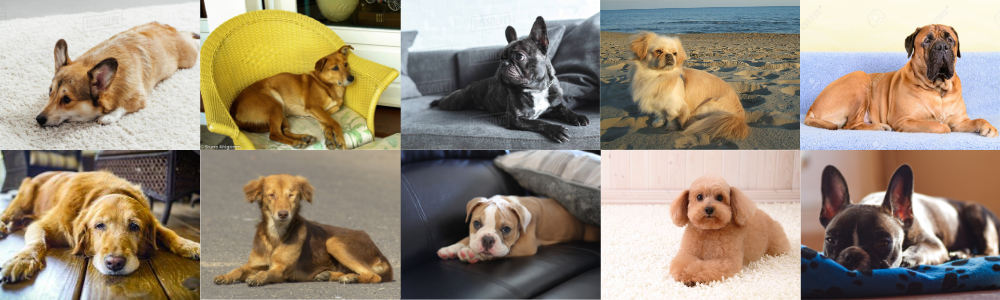
\includegraphics [width=\textwidth] {laying_perfect_dogs}
  \caption{Идеально лежащие собаки} 
  \label{img:laying_perfect_dogs}  
\end{figure}

Это как раз то, что было нужно. Все собаки были на достаточном отдалении от камеры и все их конечности были хорошо видны, т.е. не загораживали друг друга.

\subsection{Получение датасета}\label{sect3_3_1}

На основе увиденного, было принято решение собрать по этим эталонам больше собак, хотя бы по 500 на класс. В дальнейшем оказалось, что уверенность нейронной сети - относительный параметр. Классы, которые нейронная сеть легко классифицирует обладают достаточной дисперсией вокруг 100\% вероятности. На практике это означало, что для хорошо подготовленного класса сидячих собак, можно было опустить уверенность сети до 93\% чтобы получить схожую вероятность получить эталонные кадры.

Собственно, каждый класс датасета был дополнен лучшими его представителями до одинакового количества изображений на класс. После этого изображения прошли дополнительную чистку на наличие спорных изображений. Это позволило поднять количество изображений до примерно 300 на класс.

% спорное изображение, не понятно собака стоит или сидит.
\begin{figure}[ht] 
  \center
  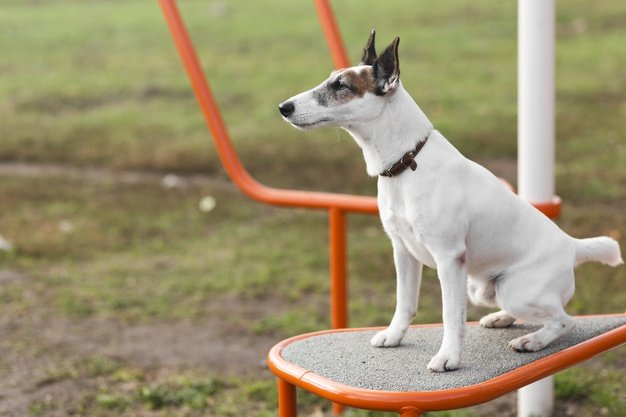
\includegraphics [width=\textwidth*2/3] {sit_or_stand}
  \caption{Спорное изображение, не понятно собака стоит или сидит.} 
  \label{img:laying_perfect_dogs}  
\end{figure}

Окончательно поставить точку в количестве данных позволил плохо размеченный OpenImageDataset. В нём все 20000 изображений были отклассифицированы, и лучшие его представители тоже были отобраны, а затем вручную проверены. В итоге это позволило добавить ещё по 200 изображений на класс до общих 500. Получается, выход достаточно небольшой: из 20000 изображений, частью нового датасета стали всего лишь 1500. (напомним, что предыдущие изображения были тоже взяты из этого датасета).
Недостающие изображения сидячих собак были дополнены 100 фотографиями сидячих лабрадоров из flickr. Маленький сет практически идеален, поэтому его можно брать без дополнительной проверки.

\subsection{Результаты на новых данных}\label{sect3_3_2}

Наконец, многообещающий новый датасет можно проверить на практике. Даже когда он ещё не до конца был собран, было ясно что его достаточно просто будет классифицировать.

Для классификации была взята модель MobileNet\cite{mobilenet} с изменённой головой классификации. Вместо ReLU на предпоследнем полносвязном слое использовалась функция активации TanH, а также DropOut\cite{dropout} с вероятностью 20\% и BatchNorm \cite{batchnorm} - нормализация в пределах текущего фрагмента данных для обучения, с целью не допустить переобучения на столь маленьком наборе данных.

В результате получилась модель, которая с 96\% валидационной точностью классифицировала этот датасет. Благодаря мерам по регуляризации точность на отдельной выборке данных была схожа с точностью на обучающих данных.

Хорошие новости:
\begin{itemize}
    \item Есть датасет, на котором принципиально возможно обучить нейронную сеть
    \item Точность классификации достаточна для поставленной задачи
    \item Создан способ, позволяющий получить датасет любого размера. Требуется только однократная валидация человеком
\end{itemize}


Плохие новости:
\begin{itemize}
    \item Нейронная сеть в состоянии работать только при удовлетворении множества условий, о которых будет рассказано далее
    \item Датасет не предусматривает наличие пограничных случаев - например, когда собака сидит, но не совсем обычным образом
    \item Не все позы собаки можно поделить на "сидит", "стоит" и "лежит". Собаки часто лежат на спине, на боку, лежат с поднятой головой итд. Собаки ещё бегут, прыгают и кружатся - все эти случаи не попадают под нашу классификацию.
\end{itemize}

Итог. Даже при наличии всех недостатков, лучше иметь систему, которая хорошо работает при известных случаях, чем ту, которая совершенно не работает при каждом случае. \cite{karpathy}